% Created 2021-05-07 Fri 11:16
% Intended LaTeX compiler: pdflatex

\documentclass[a4paper,12pt]{article}
\usepackage[margin=2cm]{geometry}

\usepackage{hyperref}
\usepackage[utf8]{inputenc}
\usepackage{fixltx2e}
\usepackage{graphicx}
\usepackage{longtable}
\usepackage{float}
\usepackage{wrapfig}
\usepackage{rotating}
\usepackage[normalem]{ulem}
\usepackage{amsmath}
\usepackage{textcomp}
\usepackage{marvosym}
\usepackage{wasysym}
\usepackage{multicol}
\usepackage{amssymb}
\tolerance=1000
\usepackage{listings}
\usepackage{titlesec}
\newcommand{\sectionbreak}{\clearpage}
\usepackage[scaled]{helvet}
\usepackage{courier}
\linespread{1.10}
\usepackage[margin=1.0in]{geometry}
\usepackage[numbers,sort&compress,square]{natbib}
\usepackage{glossaries}
\makeglossaries
\usepackage{setspace} \singlespacing
\usepackage{enumitem}
\setlist[itemize]{noitemsep, topsep=0pt}
\setlist[enumerate]{noitemsep, topsep=0pt}
\setlength\arrayrulewidth{0.7pt} % width of table line
\usepackage[english]{babel}
\addto\captionsenglish{\renewcommand\contentsname{Outline}}
\hypersetup{linktoc = all, colorlinks = true, urlcolor = DodgerBlue4, citecolor = PaleGreen1, linkcolor = black}
\usepackage[UTF8, heading]{ctex}
\usepackage{xltxtra}
\usepackage{xeCJK}
\usepackage{lmodern}
\usepackage{verbatim}
\usepackage{float}
\usepackage{tikz}
\usepackage{wrapfig}
\usepackage{soul}
\usepackage{textcomp}
\usepackage{algorithm}
\usepackage{algorithmic}
\usepackage{marvosym}
\usepackage{wasysym}
\usepackage{natbib}
\usepackage{fancyhdr}
\usepackage{fontspec,xunicode,xltxtra}
\usepackage{CJKnumb}
\usepackage{amsfonts}
\usepackage[default]{sourcecodepro}
\usepackage[T1]{fontenc}
\setCJKmainfont{SimSun} % 設置缺省中文字體
\setmainfont[Scale=0.8]{Times New Roman} % 英文襯線字體
\setsansfont[Scale=0.8]{Source Code Pro} % 英文無襯線字體
\setmonofont[Scale=0.8]{Source Code Pro} % 英文等寬字體
\setCJKmainfont[Scale=0.9]{Adobe Heiti Std} % 中文字體
\setCJKmonofont[Scale=0.9]{Adobe Heiti Std}
\usepackage{color}
\RequirePackage{fancyvrb}
\usepackage{placeins}
\hypersetup{pdfauthor={Name}}
\definecolor{dkgreen}{rgb}{0,0.6,0}
\definecolor{dred}{rgb}{0.545,0,0}
\definecolor{dblue}{rgb}{0,0,0.545}
\definecolor{lgrey}{rgb}{0.9,0.9,0.9}
\definecolor{gray}{rgb}{0.4,0.4,0.4}
\definecolor{darkblue}{rgb}{0.0,0.0,0.6}
\definecolor{bubbles}{rgb}{0.91, 1.0, 1.0}
\definecolor{foreground}{RGB}{220,220,204} % 淺灰
\definecolor{background}{RGB}{62,62,62} % 淺黑
\definecolor{preprocess}{RGB}{250,187,249} % 淺紫
\definecolor{var}{RGB}{239,224,174} % 淺肉色
\definecolor{string}{RGB}{154,150,230} % 淺紫色
\definecolor{type}{RGB}{225,225,116} % 淺黃
\definecolor{function}{RGB}{140,206,211} % 淺天藍
\definecolor{keyword}{RGB}{239,224,174} % 淺肉色
\definecolor{comment}{RGB}{180,98,4} % 深褐色
\definecolor{doc}{RGB}{175,215,175} % 淺鉛綠
\definecolor{comdil}{RGB}{111,128,111} % 深灰
\definecolor{constant}{RGB}{220,162,170} % 粉紅
\lstdefinelanguage{cpp}{ %%定義語言style
backgroundcolor=\color{bubbles},
basicstyle=\footnotesize \ttfamily \color{dblue},
breakatwhitespace=false,
breaklines=true,
captionpos=b,
comment=[l]{\#},
morecomment=[s]{/*}{*/},
commentstyle=\color{comment} \slshape \small \itshape,
ndkeywords={print, printf, repeat, struct, enum, case, switch, func, let, var, boolean, throw, import, typeof, null, catch, switch, for, in, int, str, float, self, return, class, if ,elif, endif, while, do, else, True, False , catch, def},
ndkeywordstyle=\color{dred} \bfseries \small \mono,
identifierstyle=\color{black},
deletekeywords={...},
escapeinside={\%*}{*)},
frame=single,
frameround=tttt,
framesep=0pt,
rulecolor=\color{background},
morekeywords={BRIEFDescriptorConfig,string,TiXmlNode,DetectorDescriptorConfigContainer,istringstream,cerr,exit},
identifierstyle=\color{black},
stringstyle=\color{blue},
rulecolor=\color{black},
showspaces=false,
showstringspaces=false,
showtabs=true,
stepnumber=1,
tabsize=5,
title=\lstname,
}
\lstdefinelanguage{shell}{
backgroundcolor=\color{keyword},
basicstyle=\footnotesize \ttfamily \color{dblue} \small \mono \bfseries,
breakatwhitespace=false,
breaklines=true,
captionpos=b,
comment=[l]{\#},
morecomment=[s]{/*}{*/},
commentstyle=\color{comment} \slshape \small \itshape,
identifierstyle=\color{black},
deletekeywords={...},
escapeinside={\%*}{*)},
frame=single,
frameround=tttt,
framesep=0pt,
rulecolor=\color{background},
morekeywords={BRIEFDescriptorConfig,string,TiXmlNode,DetectorDescriptorConfigContainer,istringstream,cerr,exit},
identifierstyle=\color{black},
stringstyle=\color{blue},
rulecolor=\color{black},
showspaces=false,
showstringspaces=false,
showtabs=false,
stepnumber=1,
tabsize=5,
title=\lstname,
}
\author{Yung Chin, Yen}
\date{\today}
\title{AI for TNFSH: 從入門到入土}
\begin{document}

\maketitle
\setcounter{tocdepth}{2}
\tableofcontents

\newpage

\section{人工智慧簡介}
\label{sec:org8063307}
\subsection{Chat robot}
\label{sec:orgfe4f024}
\begin{enumerate}
\item ELIZA
\label{sec:org0fc2be1}
\begin{itemize}
\item \href{https://en.wikipedia.org/wiki/ELIZA\#cite\_note-turing-1}{What is it}\\
\item \href{https://web.njit.edu/\~ronkowit/eliza.html}{web-based version}\\
\end{itemize}
\item ALICE
\label{sec:org3e0d1bf}
\begin{itemize}
\item \href{https://en.wikipedia.org/wiki/Artificial\_Linguistic\_Internet\_Computer\_Entity}{About ALICE}\\
\item \href{http://www.mfellmann.net/content/alice.html}{web-based version}\\
\end{itemize}
\item Mitsuku
\label{sec:org4da6a7b}
\begin{itemize}
\item \href{https://en.wikipedia.org/wiki/Mitsuku}{About Mitsuku}\\
\item \href{https://chat.kuki.ai/}{Try it}\\
\end{itemize}
\newpage
\end{enumerate}

\section{背景知識}
\label{sec:org2c4eab9}
\newpage

\section{監督式學習}
\label{sec:org3774e52}
\subsection{最短距離分類器}
\label{sec:org51a21a5}
\lstset{breaklines=true,language=Python,label= ,caption= ,captionpos=b,firstnumber=1,numbers=left}
\begin{lstlisting}
import math
#from statistics import mean



# importing reduce()
from functools import reduce

def Average(lst):
    avgx = 0
    avgy = 0
    for (x, y) in lst:
        avgx += x
        avgy += y
    return avgx/len(lst), avgy/len(lst)

def ed(lst, x, y):
    dist = 0
    for (lx, ly) in lst:
        dist += (x - lx)*(x - lx) + (y - ly)*(y - ly)
    return math.sqrt(dist)

groupA = [[4, 6] ,[5,7] ,[5,8] ,[5.8,6] ,[6,6] ,[6,7] ,[7,5] ,[7,7] ,[8,4] ,[9,5]]
groupB = [[2,2] ,[4,2] ,[4,4] ,[5,4] ,[5,3] ,[6,2]]

tarx = 5
tary = 5

centerX, centerY = Average(groupA)
sdA = (tarx - centerX)*(tarx - centerX)
centerX, centerY = Average(groupB)
sdB = (tarx - centerX)*(tarx - centerX)

if sdA < sdB:
    print("A")
else:
    print("B")

print(ed(groupA, tarx, tary))
print(ed(groupB, tarx, tary))


\end{lstlisting}

\begin{verbatim}
B
7.851114570556208
6.708203932499369
\end{verbatim}

\subsection{KNN實作}
\label{sec:orge1334df}
K-NearestNeighbor分類算法是機器學習裡監督類學習中最簡單的方法之一,由Cover和Hart在1968年提出。kNN算法的核心思想是如果一個樣本在特徵空間中的k個最相鄰的樣本中的大多數屬於某一個類別，則該樣本也屬於這個類別，並具有這個類別上樣本的特性。\\

KNN為 lazy learner(惰性學習器)的典型例子，所謂惰性是指它不會從「訓練數據集」中學習出「判別函數」(discriminative function)，它的作法是把「訓練數據集」記憶起來。其步驟如下：\\
\begin{enumerate}
\item 選定 k 的值和一個「距離度量」(distance metric)。\\
\item 找出 k 個想要分類的、最相近的鄰近樣本。\\
\item 以多數決的方式指定類別標籤。\\
\end{enumerate}

\begin{enumerate}
\item 鳶尾花分類問題
\label{sec:orga1aeac6}
\begin{enumerate}
\item DataSet
\label{sec:org55b5372}
收集了3種鳶尾花的四個特徵，分別是花萼(sepal)長寬、花瓣(petal)長寬度，以及對應的鳶尾花種類。\\
\begin{figure}[htbp]
\centering
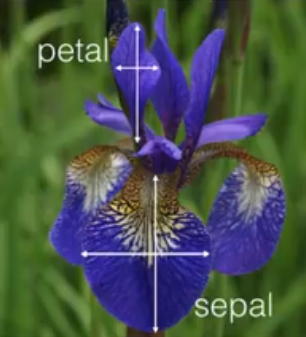
\includegraphics[width=300]{images/iris-1.png}
\caption{\label{fig:iris-1}鳶尾花的花萼與花瓣}
\end{figure}
\item Mission
\label{sec:org09a080c}
輸入花萼和花瓣數據後，推測所屬的鳶尾花類型。\\
\begin{figure}[htbp]
\centering
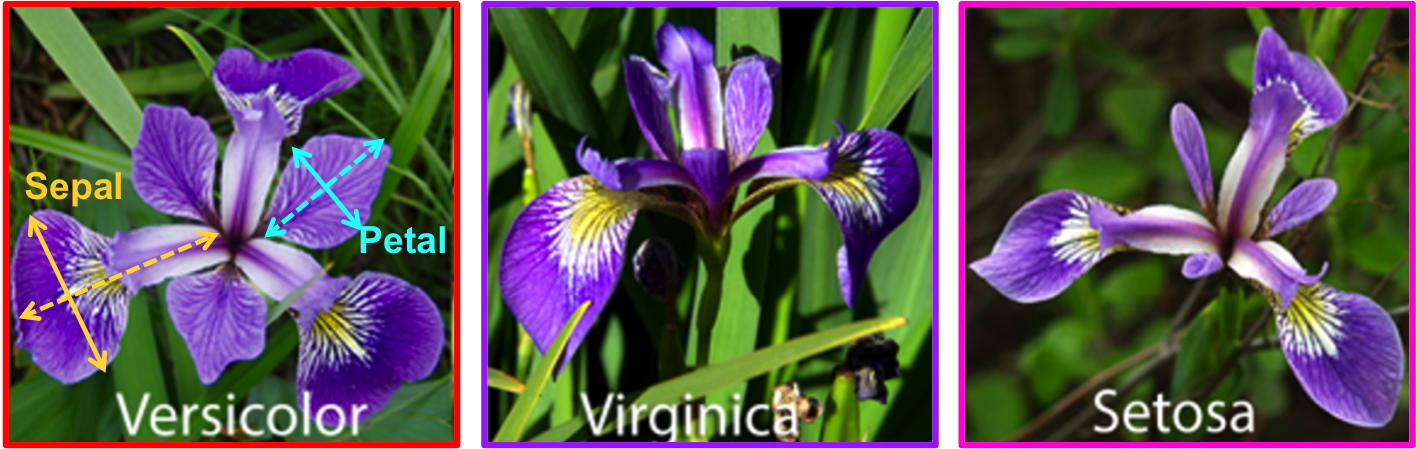
\includegraphics[width=400]{images/iris-2.png}
\caption{\label{fig:Name}三種鳶尾花}
\end{figure}
\end{enumerate}

\item 實作
\label{sec:org93eba85}
\begin{enumerate}
\item 讀取資料集\\
\lstset{breaklines=true,language=Python,label= ,caption= ,captionpos=b,firstnumber=1,numbers=left}
\begin{lstlisting}
from sklearn import datasets

# 讀入資料
iris = datasets.load_iris()
print(iris.DESCR)
\end{lstlisting}

\item 取出特徵與標籤\\
\lstset{breaklines=true,language=Python,label= ,caption= ,captionpos=b,firstnumber=1,numbers=left}
\begin{lstlisting}
x = iris.data
y = iris.target
print(x[:5])
print(y[:5])
\end{lstlisting}
\item 資料觀察\\
\lstset{breaklines=true,language=Python,label= ,caption= ,captionpos=b,firstnumber=1,numbers=left}
\begin{lstlisting}
import matplotlib.pyplot as plt
import pandas as pd
import seaborn as sns
#把nupmy ndarray轉為pandas dataFrame,加上columns title
npx = pd.DataFrame(x, columns=['fac1','fac2','fac3','fac4'])
npy = pd.DataFrame(y.astype(int), columns=['category'])
#合併
dataPD = pd.concat([npx, npy], axis=1)
print(dataPD)
# 畫圖
sns.lmplot('fac1', 'fac2', data=dataPD, hue='category', fit_reg=False)
plt.show()
\end{lstlisting}

\item 分割資料集\\
\lstset{breaklines=true,language=Python,label= ,caption= ,captionpos=b,firstnumber=1,numbers=left}
\begin{lstlisting}
from sklearn.model_selection import train_test_split
# 劃分資料集
x_train, x_test, y_train, y_test = train_test_split(iris.data, iris.target, random_state=6)
\end{lstlisting}

\begin{itemize}
\item train\_test\_split()\\
所接受的變數其實非常單純，基本上為 3 項：『原始的資料』、『Seed』、『比例』\\
\begin{enumerate}
\item 原始的資料：就如同上方的 data 一般，是我們打算切成 Training data 以及 Test data 的原始資料\\
\item Seed： 亂數種子，可以固定我們切割資料的結果\\
\item 比例：可以設定 train\_size 或 test\_size，只要設定一邊即可，範圍在 [0-1] 之間\\
\end{enumerate}
\item scikit-learn.org: sklearn.model\_selection.train\_test\_split\\

Split arrays or matrices into random train and test subsets\\

Quick utility that wraps input validation and next(ShuffleSplit().split(X, y)) and application to input data into a single call for splitting (and optionally subsampling) data in a oneliner.\\
\lstset{breaklines=true,language=Python,label= ,caption= ,captionpos=b,firstnumber=1,numbers=left}
\begin{lstlisting}
 sklearn.model_selection.train_test_split(*arrays, test_size=None, train_size=None, random_state=None, shuffle=True, stratify=None)[source]
\end{lstlisting}

\begin{itemize}
\item \href{https://scikit-learn.org/stable/modules/generated/sklearn.model\_selection.train\_test\_split.html}{online docs}\\
\end{itemize}
\end{itemize}

\item 資料標準化\\
\lstset{breaklines=true,language=Python,label= ,caption= ,captionpos=b,firstnumber=1,numbers=left}
\begin{lstlisting}
# 將資料標準化: 利用preprocessing模組裡的StandardScaler類別
from sklearn.preprocessing import StandardScaler
# 利用fit方法，對X_train中每個特徵值估平均數和標準差
# 然後對每個特徵值進行標準化(train和test都要做)
# 特徵工程：標準化
transfer = StandardScaler()
x_train = transfer.fit_transform(x_train)
x_test = transfer.fit_transform(x_test)
\end{lstlisting}

\item 分類\\
\lstset{breaklines=true,language=Python,label= ,caption= ,captionpos=b,firstnumber=1,numbers=left}
\begin{lstlisting}
from sklearn.neighbors import KNeighborsClassifier
# KNN 分類器
estimator = KNeighborsClassifier(n_neighbors=1)
estimator.fit(x_train, y_train)

# 模型評估
# 方法一：直接對比真實值和預測值
y_predict = estimator.predict(x_test)
print('y_predict：\n', y_predict)
print('直接對比真實值和預測值:\n', y_test == y_predict)

# 方法二：計算準確率
score = estimator.score(x_test, y_test)
print('準確率:\n', score)
\end{lstlisting}
\end{enumerate}

\item 作業
\label{sec:org8f91373}
修改上述程式碼，以折線圖表示K值與KNN預測準確度間的關係。\\
\end{enumerate}

\subsection{決策樹實作}
\label{sec:org414101b}
一棵複雜的決策樹\\
\begin{figure}[htbp]
\centering
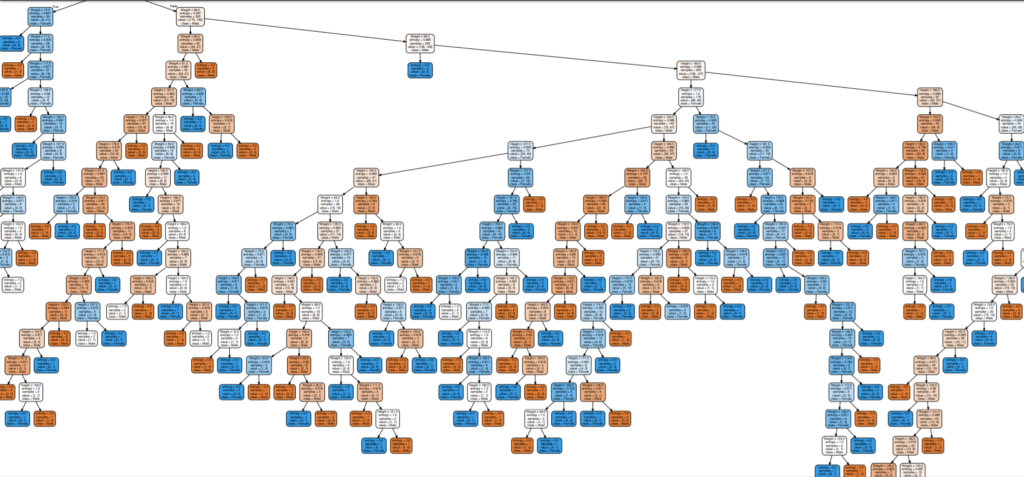
\includegraphics[width=500]{images/SBQNWUA1dDtFsMHv.png}
\caption{\label{fig:Name}Caption}
\end{figure}
\begin{enumerate}
\item iris
\label{sec:org2c6fd3a}
\lstset{breaklines=true,language=Python,label= ,caption= ,captionpos=b,firstnumber=1,numbers=left}
\begin{lstlisting}
from sklearn.datasets import load_iris
from sklearn import tree
from sklearn.model_selection import train_test_split

# Load in our dataset
# # 讀入鳶尾花資料
iris = load_iris()
iris_x = iris.data
iris_y = iris.target

# 切分訓練與測試資料
train_x, test_x, train_y, test_y = train_test_split(iris_x, iris_y, test_size = 0.3)

# 建立分類器
# Initialize our decision tree object
classification_tree = tree.DecisionTreeClassifier(criterion = "entropy")

# Train our decision tree (tree induction + pruning)
classification_tree = classification_tree.fit(iris_x, iris_y)

# 預測
test_y_predicted = classification_tree.predict(test_x)
print(test_y_predicted)

# 標準答案
print(test_y)


print('得分:',classification_tree.score(iris_x, iris_y))
import graphviz

import pydot
import matplotlib.pyplot as plt
plt.clf()
dot_data = tree.export_graphviz(classification_tree, out_file=None,
                     feature_names=iris.feature_names,
                     class_names=iris.target_names,
                     filled=True, rounded=True,
                     special_characters=True)
graph = graphviz.Source(dot_data)
#graph.render("images/DecisionTree.png", view=True)
graph.format = 'png'
graph.render('images/DecisionTree')
#plt.savefig('images/DecisionTree.png', dpi=300)

\end{lstlisting}

\begin{verbatim}
[1 0 0 2 2 2 0 2 2 1 1 1 1 2 0 1 2 1 2 1 0 1 2 1 1 2 2 0 2 2 2 2 1 0 1 1 2
 2 2 0 2 1 1 2 0]
[1 0 0 2 2 2 0 2 2 1 1 1 1 2 0 1 2 1 2 1 0 1 2 1 1 2 2 0 2 2 2 2 1 0 1 1 2
 2 2 0 2 1 1 2 0]
得分: 1.0
\end{verbatim}


\begin{figure}[htbp]
\centering

\includegraphics[width=500]{images/DecisionTree.png}
\caption{\label{fig:Name}Decision Tree}
\end{figure}
\item bank-loan\footnote{\href{https://towardsai.net/p/programming/decision-trees-explained-with-a-practical-example-fe47872d3b53}{Decision Trees Explained With a Practical Example}\\}
\label{sec:orgf3aa719}
\begin{enumerate}
\item Load the data and finish the cleaning process\\

\lstset{breaklines=true,language=Python,label= ,caption= ,captionpos=b,firstnumber=1,numbers=left}
\begin{lstlisting}
#the dataset is available on kaggle too
train = pd.read_csv('/kaggle/input/bank-loan2/madfhantr.csv')

#check for missing values
train.isnull().sum()
\end{lstlisting}

There are two possible ways to either fill the null values with some value or drop all the missing values(I dropped all the missing values).\\

If you look at the original dataset’s shape, it is (614,13), and the new data-set after dropping the null values is (480,13).\\
\lstset{breaklines=true,language=Python,label= ,caption= ,captionpos=b,firstnumber=1,numbers=left}
\begin{lstlisting}
train.dropna(inplace=True)
\end{lstlisting}

\item Take a Look at the data-set\\
We found there are many categorical values in the dataset\\
Howevern, The decision tree does not support categorical data as features.\\

So the optimal step to take at this point is you can use feature engineering techniques like label encoding and one hot label encoding.\\
\lstset{breaklines=true,language=Python,label= ,caption= ,captionpos=b,firstnumber=1,numbers=left}
\begin{lstlisting}
# I selected few of the columns from the dataset for this tutorial
train = train[['Gender','Married','Education','Self_Employed','Credit_History','Loan_Status']]

train['Gender']=train['Gender'].replace(to_replace='Male',value='1')
train['Gender']=train['Gender'].replace(to_replace='Female',value='0')


train['Married']=train['Married'].replace(to_replace='Yes',value='1')
train['Married']=train['Married'].replace(to_replace='No',value='0')


train['Self_Employed']=train['Self_Employed'].replace(to_replace='No',value='0')
train['Self_Employed']=train['Self_Employed'].replace(to_replace='Yes',value='1')


train['Education']=train['Education'].replace(to_replace='Graduate',value='1')
train['Education']=train['Education'].replace(to_replace='Not Graduate',value='0')
\end{lstlisting}

\item Split the data-set into train and test sets\\
\lstset{breaklines=true,language=Python,label= ,caption= ,captionpos=b,firstnumber=1,numbers=left}
\begin{lstlisting}
X = train.drop(columns=['Loan_Status'])
y = train.Loan_Status


from sklearn.model_selection import train_test_split
X_train,X_test,y_train,y_test = train_test_split(X,y,test_size=0.3,random_state=42)
\end{lstlisting}

Why should we split the data before training a machine learning algorithm?\\

Please visit \href{https://medium.com/@snji.khjuria/everything-you-need-to-know-about-train-dev-test-split-what-how-and-why-6ca17ea6f35}{Sanjeev’s article} regarding training, development, test, and splitting of the data for detailed reasoning.\\

\item Build the model and fit the train set.\\
\lstset{breaklines=true,language=Python,label= ,caption= ,captionpos=b,firstnumber=1,numbers=left}
\begin{lstlisting}
from sklearn.tree import DecisionTreeClassifier
from sklearn import tree

clf = tree.DecisionTreeClassifier(max_depth=3)
clf.fit(X_train,y_train)
\end{lstlisting}

Before we visualize the tree, let us do some calculations and find out the root node by using Entropy.\\
\begin{itemize}
\item Calculation 1: Find the Entropy of the total dataset\\

\item Calculation 2: Now find the Entropy and gain for every column\\

\item 
\end{itemize}
\item Visualize the Decision Tree\\
\lstset{breaklines=true,language=Python,label= ,caption= ,captionpos=b,firstnumber=1,numbers=left}
\begin{lstlisting}
import graphviz
dot_data = tree.export_graphviz(clf, out_file=None,
                               feature_names=['Gender','Married','Education','Self_Employed','Credit_History'],
                               class_names=['Yes','No'],filled=True,
                                rounded=True,
                              special_characters=True)
graph = graphviz.Source(dot_data)
graph.render("Gini")
graph
\end{lstlisting}

Well, it’s like we got the calculations right!\\

So the same procedure repeats until there is no possibility for further splitting.\\
\item Check the score of the model\\
\lstset{breaklines=true,language=Python,label= ,caption= ,captionpos=b,firstnumber=1,numbers=left}
\begin{lstlisting}
clf.score(X_test,y_test)
#output = 0.7986111111111112
\end{lstlisting}

We almost got 80\% percent accuracy. Which is a decent score for this type of problem statement?\\
\end{enumerate}
\begin{enumerate}
\item DEMO
\label{sec:org98e2716}
\lstset{breaklines=true,language=Python,label= ,caption= ,captionpos=b,firstnumber=1,numbers=left}
\begin{lstlisting}
import numpy as np
import pandas as pd
## 1. Load the data and finish the cleaning process
##    the dataset is available on kaggle too
train = pd.read_csv('./madfhantr.csv')

#check for missing values
train.isnull().sum()
#
train.dropna(inplace=True)
## 2. Take a Look at the data-set
# I selected few of the columns from the dataset for this tutorial
train = train[['Gender','Married','Education','Self_Employed','Credit_History','Loan_Status']]

train['Gender']=train['Gender'].replace(to_replace='Male',value='1')
train['Gender']=train['Gender'].replace(to_replace='Female',value='0')


train['Married']=train['Married'].replace(to_replace='Yes',value='1')
train['Married']=train['Married'].replace(to_replace='No',value='0')


train['Self_Employed']=train['Self_Employed'].replace(to_replace='No',value='0')
train['Self_Employed']=train['Self_Employed'].replace(to_replace='Yes',value='1')


train['Education']=train['Education'].replace(to_replace='Graduate',value='1')
train['Education']=train['Education'].replace(to_replace='Not Graduate',value='0')
## 3. Split the data-set into train and test sets
X = train.drop(columns=['Loan_Status'])
y = train.Loan_Status


from sklearn.model_selection import train_test_split
X_train,X_test,y_train,y_test = train_test_split(X,y,test_size=0.3,random_state=42)
## 4. Build the model and fit the train set.
from sklearn.tree import DecisionTreeClassifier
from sklearn import tree

clf = tree.DecisionTreeClassifier(max_depth=3)
clf = clf.fit(X_train,y_train)
print(clf.score(X_train, y_train))
## 5. Visualize the Decision Tree
import graphviz
dot_data = tree.export_graphviz(clf, out_file=None,
                               feature_names=['Gender','Married','Education','Self_Employed','Credit_History'],
                               class_names=['Yes','No'],filled=True,
                                rounded=True,
                              special_characters=True)
graph = graphviz.Source(dot_data)
#graph.render("Gini")
graph.format = 'png'
graph.render('images/DecisionTree2')
#graph
## 6. Check the score of the model
clf.score(X_test,y_test)
\end{lstlisting}

\begin{verbatim}
0.8125
\end{verbatim}

\begin{figure}[htbp]
\centering
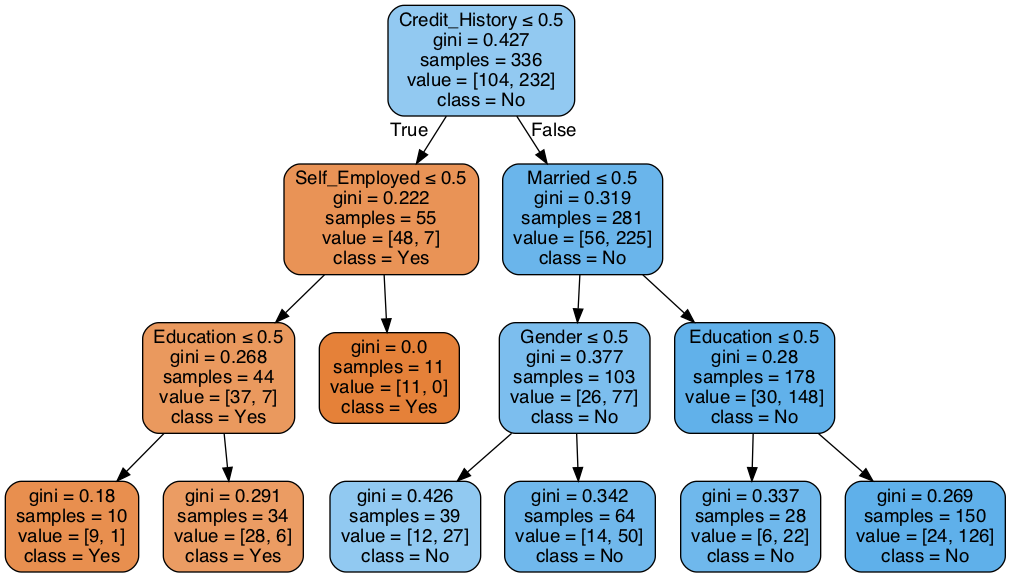
\includegraphics[width=500]{images/DecisionTree2.png}
\caption{\label{fig:tree-2}Bank Load 2}
\end{figure}
\newpage
\end{enumerate}
\end{enumerate}

\section{非監督式學習}
\label{sec:orgfc4a6ff}
\subsection{K-Means}
\label{sec:orgacda78c}
\href{https://alankrantas.medium.com/kmeans-\%E8\%83\%BD\%E5\%BE\%9E\%E8\%B3\%87\%E6\%96\%99\%E4\%B8\%AD\%E6\%89\%BE\%E5\%87\%BA-k-\%E5\%80\%8B\%E5\%88\%86\%E9\%A1\%9E\%E7\%9A\%84\%E9\%9D\%9E\%E7\%9B\%A3\%E7\%9D\%A3\%E5\%BC\%8F\%E6\%A9\%9F\%E5\%99\%A8\%E5\%AD\%B8\%E7\%BF\%92\%E6\%BC\%94\%E7\%AE\%97\%E6\%B3\%95-\%E6\%89\%80\%E4\%BB\%A5\%E5\%AE\%83\%E5\%88\%B0\%E5\%BA\%95\%E6\%9C\%89\%E5\%95\%A5\%E7\%94\%A8-\%E4\%BD\%BF\%E7\%94\%A8-scikit-learn-\%E8\%88\%87-python-5dd8c0c8b167}{KMeans：能從資料中找出 K 個分類的非監督式機器學習演算法 — — 所以它到底有啥用？}\\
\lstset{breaklines=true,language=Python,label= ,caption= ,captionpos=b,firstnumber=1,numbers=left}
\begin{lstlisting}
sklearn.datasets.samples_generator import make_blobs
X, y_true = make_blobs(n_samples=300, centers=4, cluster_std=0.60, random_state=0)
plt.scatter(X[:, 0], X[:, 1], s=50);
plt.show()

\end{lstlisting}

\lstset{breaklines=true,language=Python,label= ,caption= ,captionpos=b,firstnumber=1,numbers=left}
\begin{lstlisting}
from sklearn.cluster import KMeans

kmeans = KMeans(n_clusters=3)

kmeans.fit(X)
cluster = kmeans.predict(X)

plt.scatter(X[:,0], X[:,1], c=cluster, cmap=plt.cm.Set1)

plt.show()
\end{lstlisting}

\subsection{Hierarchical clustering}
\label{sec:org4621041}
階層式分群法（Hierarchical Clustering）\\
階層式分群法透過一種階層架構的方式，將資料層層反覆地進行分裂或聚合，以產生最後的樹狀結構，常見的方式有兩種：\\

\begin{enumerate}
\item 聚合式階層分群法 (Bottom-up, agglomerative) : 如果採用聚合的方式，階層式分群法可由樹狀結構的底部開始，將資料或群聚逐次合併。
\label{sec:org10c4eff}
定義兩個群聚之間的距離\\
\begin{itemize}
\item 單一連結聚合演算法(single-linkage agglomerative algorithm)：群聚與群聚間的距離可以定義為不同群聚中最接近兩點間的距離。\\
\item 完整連結聚合演算法(complete-linkage agglomerative algorithm）：群聚間的距離定義為不同群聚中最遠兩點間的距離，這樣可以保證這兩個集合合併後, 任何一對的距離不會大於 d。\\
\item 平均連結聚合演算法(average-linkage agglomerative algorithm)：群聚間的距離定義為不同群聚間各點與各點間距離總和的平均。沃德法（Ward's method）：群聚間的距離定義為在將兩群合併後，各點到合併後的群中心的距離平方和。\\
\end{itemize}
\lstset{breaklines=true,language=Python,label= ,caption= ,captionpos=b,firstnumber=1,numbers=left}
\begin{lstlisting}
import scipy.cluster.hierarchy as sch
dis=sch.linkage(X,metric='euclidean',method='ward')
#metric: 距離的計算方式
#method: 群與群之間的計算方式，”single”, “complete”, “average”, “weighted”, “centroid”, “median”, “ward”

sch.dendrogram(dis)
plt.title('Hierarchical Clustering')
plt.show()
\end{lstlisting}

Agglomerative Clustering Sample\\
\lstset{breaklines=true,language=Python,label= ,caption= ,captionpos=b,firstnumber=1,numbers=left}
\begin{lstlisting}
from sklearn.cluster import AgglomerativeClustering
import numpy as np

# randomly chosen dataset
X = np.array([[1, 2], [1, 4], [1, 0],
              [4, 2], [4, 4], [4, 0]])

# here we need to mention the number of clusters
# otherwise the result will be a single cluster
# containing all the data
clustering = AgglomerativeClustering(n_clusters = 2).fit(X)

# print the class labels
print(clustering.labels_)
\end{lstlisting}

\begin{verbatim}
[1 1 1 0 0 0]
\end{verbatim}

\begin{enumerate}
\item 利用距離決定群數，或直接給定群數。
\label{sec:org8818b94}
建構好聚落樹狀圖後，我們可以依照距離的切割來進行分類，也可以直接給定想要分類的群數，讓系統自動切割到相對應的距離。\\
\begin{itemize}
\item 距離切割\\
所給出的樹狀圖，y軸代表距離，我們可以用特徵之間的距離進行分群的切割。\\
\lstset{breaklines=true,language=Python,label= ,caption= ,captionpos=b,firstnumber=1,numbers=left}
\begin{lstlisting}
max_dis=5
clusters=sch.fcluster(dis,max_dis,criterion='distance')
\end{lstlisting}

\item 直接給定群數\\
同時，我們也可以像sklearn一樣，直接給定我們所想要分出的群數。\\
\lstset{breaklines=true,language=Python,label= ,caption= ,captionpos=b,firstnumber=1,numbers=left}
\begin{lstlisting}
k=5
clusters=sch.fcluster(dis,k,criterion='maxclust')
\end{lstlisting}
\end{itemize}

\item 如何評估最佳分群數:K
\label{sec:org6ab2432}
\begin{itemize}
\item \href{https://jimmy-huang.medium.com/kmeans\%E5\%88\%86\%E7\%BE\%A4\%E6\%BC\%94\%E7\%AE\%97\%E6\%B3\%95-\%E8\%88\%87-silhouette-\%E8\%BC\%AA\%E5\%BB\%93\%E5\%88\%86\%E6\%9E\%90-8be17e634589}{Kmeans分群演算法 與 Silhouette 輪廓分析}\\
\item \href{https://www.geeksforgeeks.org/implementing-agglomerative-clustering-using-sklearn/}{Implementing Agglomerative Clustering using Sklearn}\\
\end{itemize}
\end{enumerate}
\item 分裂式階層分群法 (Top-down, divisible) : 如果採用分裂的方式，則由樹狀結構的頂端開始，將群聚逐次分裂。
\label{sec:orge5169f4}
Divisive clustering : Also known as top-down approach. This algorithm also does not require to prespecify the number of clusters. Top-down clustering requires a method for splitting a cluster that contains the whole data and proceeds by splitting clusters recursively until individual data have been splitted into singleton cluster.\\
\end{enumerate}



\subsection{K-Means壓縮影像}
\label{sec:org71dbfe8}
\subsection{Hierarchical}
\label{sec:org85c00b7}
\newpage

\section{增強式學習}
\label{sec:orgf1e2947}
強化學習(Reinforcement learning, RL)是機器學習的一個子領域，在智能控制機器人及分析預測等領域有許多應用。強化學習通過與環境進行交互獲得的獎賞指導行為，目標是使智能體獲得最大的獎賞，最終開發出智能體(Agent)做出決策和控制\footnote{\href{https://blog.csdn.net/qq\_32892383/article/details/89576003}{OpenAI Gym 經典控制環境介紹——CartPole（倒立擺）}\\}。\\

對RL稍有了解的同學都知道，Exploration是一件很重要同時也很困難的事情。與其他機器學習範式相比，RL通常只知道某個動作的能得多少分，卻不知道該動作是不是最好的——這就是基於evaluate的強化學習與基於instruct的監督學習的根本區別。\\

正因如此，RL的本質決定了它極其需要Exploration，我們需要通過不斷地探索來發現更好的決策，或者至少證明當前的決策是最好的——所以Exploration-Exploitation成為了強化學習領域諸個Tradeoff中最出名的一個\footnote{\href{https://kknews.cc/zh-tw/news/34mob53.html}{強化學習Exploration漫遊}\\\label{org0d3d039}}。\\

最簡單的exploration方法就是epsilon-greedy，即設置一個探索率epsilon來平衡兩者的關係——在大部分時間裡採用現階段最優策略，在少部分時間裡實現探索。\\

Epsilon-greedy很簡單，它根本不會考慮更加有針對性的探索機制，它僅僅是在純貪心的基礎上加入了一定機率的uniform噪聲——所以epsilon-greedy又被稱為Naive Exploration\textsuperscript{\ref{org0d3d039}}。\\
\subsection{AgentBellman Equation}
\label{sec:org046ae49}
\newpage
\begin{enumerate}
\item Bellman Equation
\label{sec:org85630f3}
\item Markov Decision Process / MDP
\label{sec:orga4757e5}
\end{enumerate}
\subsection{Q-Learning}
\label{sec:org77a15ce}
\subsection{實作: CartPole}
\label{sec:orgb2da449}
\begin{enumerate}
\item Gym
\label{sec:org6fc58a5}
Gym是一個研究和開發強化學習相關算法的仿真平台，無需智能體先驗知識，並兼容常見的數值運算庫如 TensorFlow、Theano等。OpenAI Gym由以下兩部分組成：\\
\begin{itemize}
\item Gym開源庫：測試問題的集合。當你測試強化學習的時候，測試問題就是環境，比如機器人玩遊戲，環境的集合就是遊戲的畫面。這些環境有一個公共的接口，允許用戶設計通用的算法。\\
\item OpenAI Gym服務：提供一個站點和API（比如經典控制問題：CartPole-v0），允許用戶對他們的測試結果進行比較。\\
\end{itemize}

簡單來說OpenAI Gym提供了許多問題和環境（或遊戲）的接口，而用戶無需過多瞭解遊戲的內部實現，通過簡單地調用就可以用來測試和仿真。\\
\item Environment:
\label{sec:orgd506456}
\begin{enumerate}
\item Launch ANACONDA NAVIGATOR\\
\item Launch Spyder\\
\item pip install --user gym\\
\item pip install --user pyglet==1.5.11\\
\end{enumerate}
\item Demo code
\label{sec:org16f1a43}
\lstset{breaklines=true,language=Python,label= ,caption= ,captionpos=b,firstnumber=1,numbers=left}
\begin{lstlisting}
import gym
env = gym.make('CartPole-v0')
env.reset()
for _ in range(100):
    env.render()
    # 隨機產生下一動作
    env.step(env.action_space.sample()) # take a random action
env.close()
\end{lstlisting}
\item Gym fomulation
\label{sec:org54ba465}
\begin{itemize}
\item Agent：小車控制系統。\\
\item Environment：CartPole。\\
\item State：四種 feature：車子位置（1D）、車子速度、柱子角度、柱子角速度。\\
\item Action：將車子向左或向右控制。\\
\item Reward：每個 timestep 如果柱子還站著則 +1。如果柱子太歪或車子跑太遠就結束一回合，所以每一回合站越久總 reward 就越大。\\
\end{itemize}
\item OpenAI Gym
\label{sec:org3bb93c0}
列出可用的遊戲\\
\lstset{breaklines=true,language="exports,label= ,caption= ,captionpos=b,numbers=none}
\begin{lstlisting}
"exports both"body
\end{lstlisting}
\item Minimum Example
\label{sec:org8c3b00a}
\lstset{breaklines=true,language=Python,label= ,caption= ,captionpos=b,firstnumber=1,numbers=left}
\begin{lstlisting}
import gym
env = gym.make('CartPole-v0')
env.reset()
for _ in range(100):
    env.render()
    env.step(env.action_space.sample()) # take a random action
env.close()
\end{lstlisting}
\item Observations
\label{sec:org88861d1}
If we ever want to do better than take random actions at each step, it’d probably be good to actually know what our actions are doing to the environment.\\

The environment’s step function returns exactly what we need. In fact, step returns four values. These are\footnote{\href{http://gym.openai.com/docs/}{Getting Started with Gym}\\}:\\
\begin{itemize}
\item observation (object): an environment-specific object representing your observation of the environment. For example, pixel data from a camera, joint angles and joint velocities of a robot, or the board state in a board game.\\
\item reward (float): amount of reward achieved by the previous action. The scale varies between environments, but the goal is always to increase your total reward.\\
\item done (boolean): whether it’s time to reset the environment again. Most (but not all) tasks are divided up into well-defined episodes, and done being True indicates the episode has terminated. (For example, perhaps the pole tipped too far, or you lost your last life.)\\
\item info (dict): diagnostic information useful for debugging. It can sometimes be useful for learning (for example, it might contain the raw probabilities behind the environment’s last state change). However, official evaluations of your agent are not allowed to use this for learning.\\
\end{itemize}

This is just an implementation of the classic “agent-environment loop”. Each timestep, the agent chooses an action, and the environment returns an observation and a reward.\\
\begin{figure}[htbp]
\centering
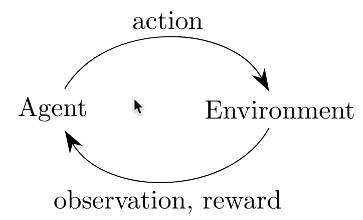
\includegraphics[width=300]{images/cartpole-cycle.jpg}
\caption{\label{fig:Name}Cartpole cycle}
\end{figure}
\item Random Action
\label{sec:orgbba2fbd}
\lstset{breaklines=true,language=Python,label= ,caption= ,captionpos=b,firstnumber=1,numbers=left}
\begin{lstlisting}
import gym
# RL 訓練長度
N_EPISODES = 1
EPISODE_LENGTH = 50

# 建立環境, 定義訓練的遊戲
env = gym.make('CartPole-v0')

# 開始訓練
reward_rec = []
for i_episode in range(N_EPISODES):
    observation = env.reset() # 把柱子擺好
    rewards = 0
    for t in range(EPISODE_LENGTH):
        env.render()

        # 隨機挑選 action，這邊是向左或向右
        action = env.action_space.sample()
        # 在環境中做出 action
        observation, reward, done, info = env.step(action)
        print(observation)

        # 累加 reward
        rewards += reward
        if done: # 回合結束，可能柱子太傾斜或車子跑遠
            print(observation[3])
            print('Episode finished after {} timesteps, total rewards {}'.format(t+1, rewards))
            reward_rec.append(rewards)
            break

env.close()
#Hide
#import matplotlib.pyplot as plt
#
#plt.clf()
#x = range(1, N_EPISODES+1)
#plt.xticks(x)
#plt.plot(x, reward_rec)
#plt.savefig('images/cart.png', dpi=300)
\end{lstlisting}

\begin{verbatim}
[-0.04725309  0.20617169 -0.03640021 -0.29821581]
[-0.04312966  0.40179309 -0.04236453 -0.60215284]
[-0.0350938   0.20728853 -0.05440758 -0.32310922]
[-0.03094803  0.40314131 -0.06086977 -0.63244161]
[-0.0228852   0.20891902 -0.0735186  -0.35953238]
[-0.01870682  0.01491496 -0.08070925 -0.09090739]
[-0.01840852  0.21109543 -0.08252739 -0.40792294]
[-0.01418661  0.01723468 -0.09068585 -0.14235703]
[-0.01384192  0.21353049 -0.09353299 -0.46221595]
[-0.00957131  0.40984127 -0.10277731 -0.78285362]
[-0.00137448  0.21627068 -0.11843439 -0.52419329]
[ 0.00295093  0.02299718 -0.12891825 -0.27105227]
[ 0.00341087 -0.17007204 -0.1343393  -0.02164878]
[ 9.43229137e-06 -3.63037241e-01 -1.34772272e-01  2.25814051e-01]
[-0.00725131 -0.16627239 -0.13025599 -0.10616002]
[-0.01057676  0.03045229 -0.13237919 -0.43693433]
[-0.00996771 -0.16257177 -0.14111788 -0.18873739]
[-0.01321915  0.03425745 -0.14489263 -0.52239742]
[-0.012534   -0.1585598  -0.15534057 -0.27865175]
[-0.0157052  -0.35116398 -0.16091361 -0.03871091]
[-0.02272848 -0.15414423 -0.16168783 -0.37752739]
[-0.02581136 -0.34664489 -0.16923838 -0.13987195]
[-0.03274426 -0.14955423 -0.17203581 -0.4808032 ]
[-0.03573534  0.04752537 -0.18165188 -0.82238816]
[-0.03478484 -0.1447085  -0.19809964 -0.59189412]
[-0.03767901  0.05255441 -0.20993752 -0.9398626 ]
-0.9398625983859829
Episode finished after 26 timesteps, total rewards 26.0
\end{verbatim}
\item Practice: 畫出統計圖表
\label{sec:orgab0fa4c}
\item Hand-Made Policy
\label{sec:orgcef2ee2}
從隨機挑選 action 進階一點，我們可以自己設計簡單的 policy。例如柱子往左傾斜，我們車子就往右，反之亦然：\\
\lstset{breaklines=true,language=Python,label= ,caption= ,captionpos=b,firstnumber=1,numbers=left}
\begin{lstlisting}
import gym

def choose_action(observation):
    pos, v, ang, rot = observation # 車位置、車速度、柱角度、柱角速度
    # 角度 < 0 選擇 action 0（車向左），否則選擇 action 1（車向右）
    return 0 if ang < 0 else 1

# RL 訓練長度
N_EPISODES = 10
EPISODE_LENGTH = 100

# 建立環境, 定義訓練的遊戲
env = gym.make('CartPole-v0')

# 開始訓練
reward_rec = []
for i_episode in range(N_EPISODES):
    observation = env.reset() # 把柱子擺好
    rewards = 0
    for t in range(EPISODE_LENGTH):
        env.render()

        # 進行自己設計的Action
        action = choose_action(observation)
        # 在環境中做出 action
        observation, reward, done, info = env.step(action)
          # 累加 reward
        rewards += reward
        if done: # 回合結束，可能柱子太傾斜或車子跑遠
            print('Episode finished after {} timesteps, total rewards {}'.format(t+1, rewards))
            reward_rec.append(rewards)
            break

env.close()

## Hide
##import matplotlib.pyplot as plt
##
##plt.clf()
##x = range(1, N_EPISODES+1)
##plt.xticks(x)
##plt.plot(x, reward_rec)
#plt.savefig('images/cart.png', dpi=300)

\end{lstlisting}

\begin{verbatim}
Episode finished after 25 timesteps, total rewards 25.0
Episode finished after 36 timesteps, total rewards 36.0
Episode finished after 47 timesteps, total rewards 47.0
Episode finished after 47 timesteps, total rewards 47.0
Episode finished after 47 timesteps, total rewards 47.0
Episode finished after 40 timesteps, total rewards 40.0
Episode finished after 48 timesteps, total rewards 48.0
Episode finished after 39 timesteps, total rewards 39.0
Episode finished after 47 timesteps, total rewards 47.0
Episode finished after 56 timesteps, total rewards 56.0
\end{verbatim}
因為沒有在學習，趨勢肯定是平的。不過平均每回合的總 reward 明顯比隨機來得好，大概能撐兩倍時間。\\
\item Hill climbing algorithm
\label{sec:org0075929}
\begin{itemize}
\item 為局部最佳解\\
\item 爬山算法的基本思路是每次迭代時給當前取得的最優權重加上一組隨機值，如果加上這組值使得有效控制倒立擺的持續時間變長了那麼就更新它爲最優權重，如果沒有得到改善就保持原來的值不變，直到迭代結束。在迭代過程中，模型的參數不斷得到優化，最終得到一組最優的權值作爲控制模型的解。其代碼如下：\\
\end{itemize}
\lstset{breaklines=true,language=Python,label= ,caption= ,captionpos=b,firstnumber=1,numbers=left}
\begin{lstlisting}
import numpy as np
import gym

def get_sum_reward_by_weights(env, weights):
    #測試不同權重的model所得到的奬勵
    observation = env.reset() #重置狀態
    rewards = 0
    for t in range(1000):
        env.render()
        # 依目前權值針對當前狀態來選action
        # 原來的做法為: action = env.action_space.sample()
        action = 1 if np.dot(weights[:4], observation) + weights[4] >= 0 else 0
        # 執行action, 取得下一步狀態
        observation, reward, done, info = env.step(action)
        rewards += reward
        if done:
            print(t)
            break
    return rewards



def get_best_result():
    np.random.seed(10)
    best_reward = 0 # 初始最佳奬勵
    best_weights = np.random.rand(5) # 初始權值為隨機值

    for iter in range(1000): #迭代100次
        cur_weights = None
        print("iteration:",iter)
        cur_weights = best_weights + np.random.normal(0, 0.1, 5) #在當前最佳權值加入隨機值
        # cur_weights = np.random.rand(5) #隨機猜測
        cur_sum_reward = get_sum_reward_by_weights(env, cur_weights)
        reward_rec.append(cur_sum_reward) #記錄用
        if cur_sum_reward > best_reward:
            best_reward = cur_sum_reward
            best_weights = cur_weights
        if best_reward >= 200:
            print(iter,":",best_reward)
            print("best_weight",best_weights)
            break;

env = gym.make("CartPole-v0")
reward_rec = []

print(get_best_result())
# 輸出統計
import matplotlib.pyplot as plt
plt.clf()
x = range(1, len(reward_rec)+1)
plt.plot(x, reward_rec)
env.close()
\end{lstlisting}

爬山算法本質是一種局部擇優的方法，效率高但因爲不是全局搜索，所以結果可能不是最優。\\
\item Q-Learning
\label{sec:org69a4183}
一個 Q-learning 非常簡單的實現法。複習一下我們在前篇提到 Q-learning，是用一個 model 來 approximate Q-value function，並藉由下面的 update rule 來訓練這個 model：\\
$$Q(S_t, a_t) = Q(s_t, a_t) + \alpha(R_{t+1} + \gamma\max_aQ(s_{s_t+1},a)-Q(s_t,a_t))$$\\
Q-table 是用 lookup table 來 approximate Q-value function，並用 Q-learning 訓練的一個方法。這個 lookup table 會將每個 state-action pair (s, a) 對應到 approximation Q(s, a)，一開始 table 裡的 Q-value 隨機設置，並在訓練過程中更新這些 Q-value。所以我們其實沒有在訓練一個 model 更新參數讓預測數值更接近 Q-value，而是直接用一個 table 記錄這些值並更新。\\

另外我們的 state 是連續值，這樣會有無限多個可能的 state-action pair，因此我們要 discretize 這些值才能建立一個 lookup table。\\

例如實作中我們把 state 的 4 個 feature (position, velocity, angle, rotation rate) 分別 discretize 成 (1, 1, 6, 3) 個 bucket，6 個 bucket 就代表 angle 的範圍 [-0.5, 0.5] 被切成 6 個區間，區間中的值都對應到相同的 discrete value。\\
\begin{enumerate}
\item 環境
\label{sec:orgfdc0335}
\begin{enumerate}
\item Observation:
\label{sec:org3ce774a}
Type: Box(4)\footnote{\href{https://github.com/openai/gym/blob/master/gym/envs/classic\_control/cartpole.py}{GitHub: openai/gym }\\\label{org43ed28a}}\\
\begin{center}
\begin{tabular}{rlrr}
Num & Observation & Min & Max\\
\hline
0 & Cart Position & -4.8 & 4.8\\
1 & Cart Velocity & -Inf & Inf\\
2 & Pole Angle & -0.418 rad (-24 deg) & 0.418 rad (24 deg)\\
3 & Pole Angular Velocity & -Inf & Inf\\
\end{tabular}
\end{center}

\item Actions
\label{sec:orged7c5d9}
Type: Discrete(2)\\
\begin{center}
\begin{tabular}{rl}
Num & Action\\
\hline
0 & Push cart to the left\\
1 & Push cart to the right\\
\end{tabular}
\end{center}
\begin{enumerate}
\item Note: The amount the velocity that is reduced or increased is not fixed; it depends on the angle the pole is pointing. This is because the center of gravity of the pole increases the amount of energy needed to move the cart underneath it\textsuperscript{\ref{org43ed28a}}.
\label{sec:orga37e492}
\end{enumerate}
\item Reward
\label{sec:org26b43ce}
Reward is 1 for every step taken, including the termination step. The threshold is 475 for v1.\\
\item Starting State:
\label{sec:org7b4bb28}
All observations are assigned a uniform random value in [-0.05..0.05]\\
\item Episode Termination:
\label{sec:org1fcd2ff}
\begin{enumerate}
\item Pole Angle is more than 12 degrees.\\
\item Cart Position is more than 2.4 (center of the cart reaches the edge of the display).\\
\item Episode length is greater than 200.\\
\end{enumerate}
Solved Requirements:\\
Considered solved when the average return is greater than or equal to 195.0 over 100 consecutive trials.\\
\end{enumerate}
\item Algorithms
\label{sec:orgb94b5fb}
\begin{figure}[htbp]
\centering
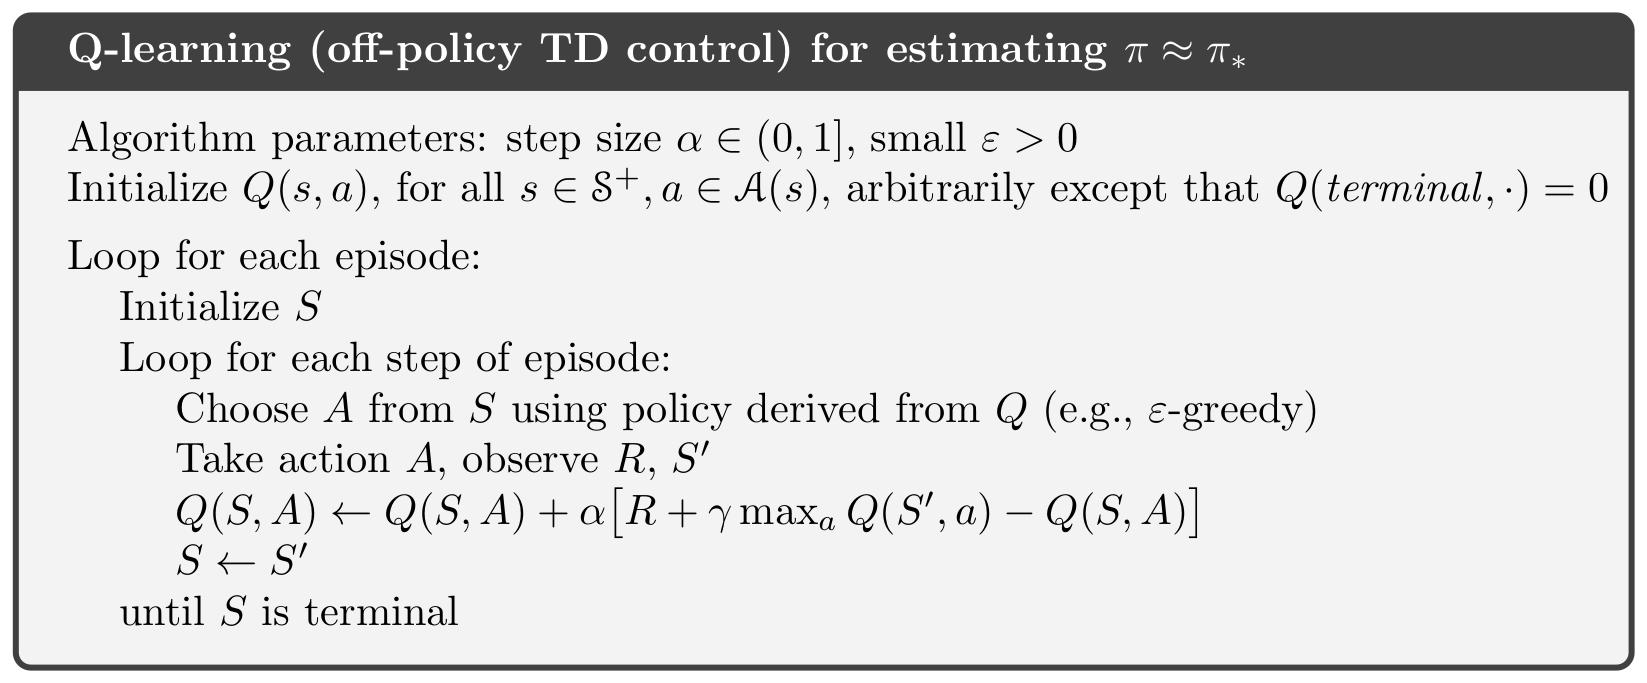
\includegraphics[width=500]{images/q-learning.png}
\caption{\label{fig:Name}Q-Learning Algorithm}
\end{figure}
在更新 Q table 時，計算 reward 不只包含採取 action \(a\)獲得的 reward \(r\)r，還包含 \(\gamma max_{a^{'}}Q(s^{'},q^{'})\)。這個概念是，agent 不僅僅看當下採取的行動帶來的好處，他也會估計到達下一個 state \(s^{'}\) 後，最多可以有多少好處（因為在\(s^{'}\)也可以採取各種 action）。\\
換句話說，這個 agent 不是一個目光如豆的 agent，他會考慮未來。因為加上了\(\gamma max_{a^{'}}Q(s^{'},q^{'})\)(當然\(\gamma\)不能是 0)，讓我們的 agent 從 會立刻吃掉棉花糖的小朋友，進化成可以晚一點再吃多一點棉花糖的小朋友，是不是很有趣呢！\\
\item Q-Table
\label{sec:org913f28b}
一個 Q-learning 非常簡單的實現法。複習一下我們在前篇提到 Q-learning，是用一個 model 來 approximate Q-value function，並藉由下面的 update rule 來訓練這個 model：\\
$$ Q(s_t,a_t) = Q(s_t,a_t) + \alpha(R_{t+1}) + \gamma \max_{a} Q(s_{t+1}, - Q(s_t,a_t)) $$\\
Q-table 是用 lookup table 來 approximate Q-value function，並用 Q-learning 訓練的一個方法。這個 lookup table 會將每個 state-action pair (s, a) 對應到 approximation Q(s, a)，一開始 table 裡的 Q-value 隨機設置，並在訓練過程中更新這些 Q-value。所以我們其實沒有在訓練一個 model 更新參數讓預測數值更接近 Q-value，而是直接用一個 table 記錄這些值並更新。\\

另外我們的 state 是連續值，這樣會有無限多個可能的 state-action pair，因此我們要 discretize 這些值才能建立一個 lookup table。\\

例如實作中我們把 state 的 4 個 feature (position, velocity, angle, rotation rate) 分別 discretize 成 (1, 1, 6, 3) 個 bucket，6 個 bucket 就代表 angle 的範圍 [-0.5, 0.5] 被切成 6 個區間，區間中的值都對應到相同的 discrete value。\\

整個 discretization 大概是這樣：\\
\lstset{breaklines=true,language=Python,label= ,caption= ,captionpos=b,firstnumber=1,numbers=left}
\begin{lstlisting}
# state bucket 設定
n_buckets = (1, 1, 6, 3)

# action 已經是 discrete value
n_actions = env.action_space.n

# 建立 Q-table
q_table = np.zeros(n_buckets + (n_actions,))

# 設定好每個 state feature 的上下界
state_bounds = list(zip(env.observation_space.low, env.observation_space.high))
state_bounds[1] = [-0.5, 0.5]
state_bounds[3] = [-math.radians(50), math.radians(50)]

# 將 env 給的 state 轉換成 discretized state
def get_state(observation, n_buckets, state_bounds):
    state = [0] * len(observation)
    for i, s in enumerate(observation):
        # 每個 feature 上界、下界
        l, u = state_bounds[i][0], state_bounds[i][1]
        if s <= l: # 低於下界屬於第 1 個 bucket
            state[i] = 0
        elif s >= u: # 高於下界屬於最後一個 bucket
            state[i] = n_buckets[i] - 1
        else: # 其他看你在哪個區間，決定你在哪個 bucket
            state[i] = int(((s - l) / (u - l)) * n_buckets[i])
    return tuple(state)
\end{lstlisting}

state\_bounds初始內容為\\
\lstset{breaklines=true,language=Python,label= ,caption= ,captionpos=b,firstnumber=1,numbers=left}
\begin{lstlisting}
[(-4.8, 4.8),
 [-0.5, 0.5],
 (-0.41887903, 0.41887903),
 [-0.8726646259971648, 0.8726646259971648]]
\end{lstlisting}

q\_table為(1, 1, 6, 3, 2)的ndarray，初始內容為\\
\lstset{breaklines=true,language=Python,label= ,caption= ,captionpos=b,firstnumber=1,numbers=left}
\begin{lstlisting}
array([[[[[0., 0.],
          [0., 0.],
          [0., 0.]],

         [[0., 0.],
          [0., 0.],
          [0., 0.]],

         [[0., 0.],
          [0., 0.],
          [0., 0.]],

         [[0., 0.],
          [0., 0.],
          [0., 0.]],

         [[0., 0.],
          [0., 0.],
          [0., 0.]],

         [[0., 0.],
          [0., 0.],
          [0., 0.]]]]])
\end{lstlisting}
\end{enumerate}
\end{enumerate}

\section{深度學習}
\label{sec:org7b20aee}
\newpage

\section{Hello world}
\label{sec:org280da05}
\newpage
\end{document}
